% !TeX root = ../车云协同液罐车防侧翻行驶规划与控制研究.tex

\chapter{引言}
\label{chap:introduction}

\section{研究背景及意义}
\label{sec:background_and_significance}

  我国危化品公路运输需求持续增长，液罐车已成为危化品运输的主要载体。统计显示，2025年我国危化品运输总额已接近3万亿元，其中超过\SI{80}{\percent}依赖液罐车公路运输\cite{qianyuyan2023}；截至2025年，危化品运输车辆总数已超过36万辆，其中液罐车接近19万辆，占比达\SI{52.8}{\percent}\cite{zhongguowuliulianhehui2022}。与此同时，液罐车运输安全问题尤为突出。2011年至2025年间，我国危化品罐车重大事故已超过1.5万起，其中\SI{78.7}{\percent}发生于液罐车行驶过程中，\SI{62.7}{\percent}由车辆侧翻引起\cite{liuhuipling2023, chengshuo2023, lijian2014,chenxiaoyong2023, wangyang2023}。在货车严重伤亡事故中，液罐车侧翻事故占比超过\SI{31}{\percent}，在液罐车单方面事故中侧翻占比接近\SI{70}{\percent}\cite{authority_tank_truck2022}。可见，侧翻已成为液罐车运行安全中的典型风险问题。

  液罐车侧翻事故往往伴随严重次生灾害，造成重大人员伤亡和财产损失。如图~\ref{fig:severe_results}所示，2020年浙江温岭G15高速液化石油气罐车侧翻爆炸事故造成20人死亡、175人受伤，并导致大量房屋倒塌和损毁\cite{wenling_accident2022}。近年来，四川江油、山东威海、广西百色、北京东六环、湖南邵阳等地亦相继发生液罐车因超速、避让、急转向等诱发的侧翻事故。由于液罐车所运载介质多为液化石油气、液化天然气、汽柴油、甲醇等易燃易爆危化品，相关事故常进一步引发泄漏、燃烧、爆炸及环境污染等严重后果\cite{qianyuyan2023, baijinghua2023}。因此，如何降低液罐车运行过程中的侧翻风险，已成为危化品道路运输安全保障中的关键问题。


  \begin{figure}
    \centering
    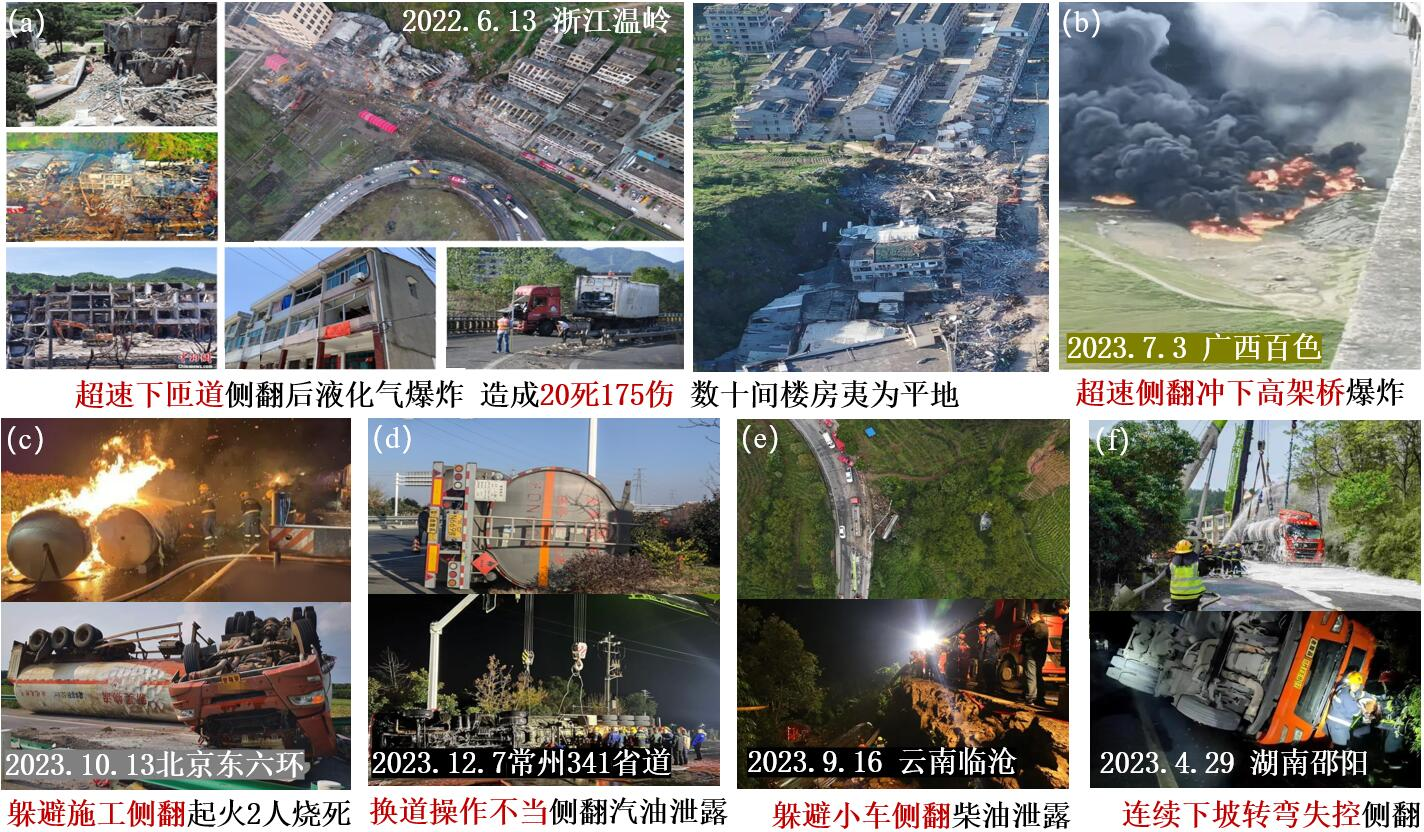
\includegraphics[width=0.9\linewidth]{fig/chap1/severe_results.jpg}
    \caption{液罐车事故及其严重后果}
    \label{fig:severe_results}
  \end{figure}

  液罐车侧翻风险的形成具有典型的多因素耦合特征，主要表现为车辆特性、单车局限与人因失误的共同作用。首先，液罐车通常需在非满载条件下运行，以避免液体膨胀和蒸汽压力升高引发泄漏或爆炸，最大允许充液量一般不得超过\SI{95}{\percent}\cite{biaozhun185642006,biaozhunR00052011}。在中低充液率条件下，罐内液体易发生显著晃动，进而降低车辆侧倾稳定性并增大侧翻风险。其次，驾驶员或单车智能系统受限于本车视角，难以充分掌握道路结构、临时施工、周车状态及行为意图等动静态交通信息，尤其在弯坡组合路段、突发干扰场景及多车交互条件下，更难以实现对风险的提前识别与规避\cite{authority_tank_truck2022}。再次，超速、疲劳驾驶以及紧急工况下的不当操纵等人因失误，也会进一步加剧车辆失稳并诱发侧翻事故。

  上述问题使自动驾驶技术成为提升液罐车行驶安全的重要潜在途径。自动驾驶系统可避免超速、疲劳驾驶等人为违规行为，依托多传感器融合提升环境感知能力，并通过优化决策与控制算法提高车辆对动态交通环境的响应速度与操纵稳定性。近年来，商用车自动驾驶技术发展迅速，已在干线物流场景中形成初步应用基础。例如，2024年卡尔动力完成2--6车混合无人化半挂车队超820万公里无事故运输\cite{kargobot2024}，小马智卡等企业的L4级自动驾驶卡车也正加快迈向规模化应用\cite{ponyai2024}。这些进展表明，自动驾驶技术为降低危化品运输中的人为失误风险提供了现实可能。

  然而，单车自动驾驶仍存在明显局限。一方面，其感知能力受限于本车视距，难以获取超视距及遮挡区域信息；另一方面，车端算力和实时优化能力有限，难以在复杂交通场景中持续执行高维预测与全局协同决策。对于液罐车而言，道路条件、周车行为与液体晃动之间存在强耦合关系，仅依靠单车智能仍难以充分应对复杂环境下的侧翻风险。

  在此背景下，车路云一体化系统（云控系统）为液罐车防侧翻提供了新的技术路径。如图~\ref{fig:cloud_platform}所示，云控系统由智能网联车辆、路侧单元、云控基础设施及定位、地图、交通管理、应急支撑等平台共同构成\cite{cuimingyang2022}，本质上属于典型的信息物理系统。通过路侧与车端协同感知、云端信息融合及虚实闭环运行，云控系统能够在更大空间范围内实现交通环境理解、预测性决策与协同控制\cite{likeqiang2020cloudcontrol}。目前，全国已有20个主要城市开展车路云一体化试点建设，表明车路云一体化已成为我国智能交通发展的重要方向\cite{gongxinbu2024pilots}。

  相较于单车智能，车云协同的优势主要体现在三个方面：其一，依托路侧与云端融合感知，可为车辆提供超视距、跨路段的全局交通信息，弥补单车感知盲区；其二，利用边缘云与云平台的并行算力，可支持更长时域、更高复杂度的风险预测与决策优化；其三，借助云端统一协调能力，可突破单车局部博弈限制，为多车场景下的整体安全与效率优化提供条件。

  \begin{figure}
      \centering
      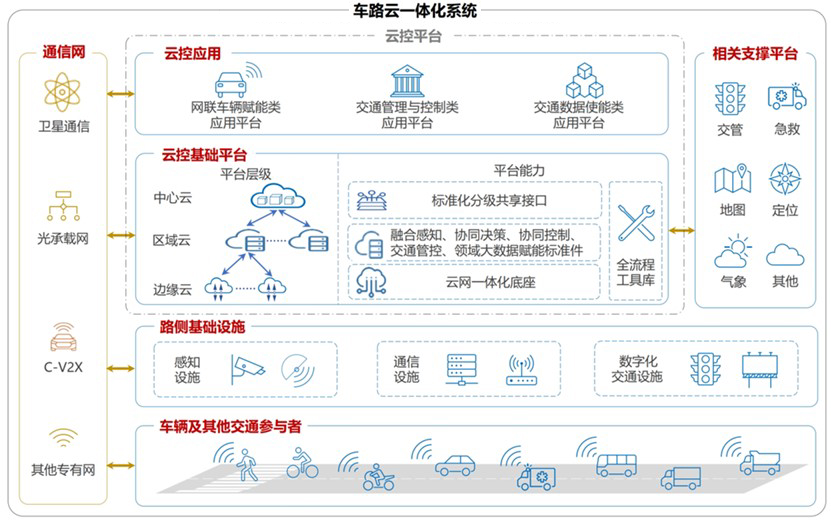
\includegraphics[width=0.9\linewidth]{fig/chap1/cloud_platform.jpg}
      \caption[车路云一体化系统架构]{车路云一体化系统架构\cite{icv2023whiteroadcloud}}
      \label{fig:cloud_platform}
  \end{figure}

  综上，液罐车侧翻风险来源于车辆非满载车液耦合特性、单车感知与决策能力不足以及人因失误等多因素共同作用。单车自动驾驶虽可在一定程度上缓解人为失误和局部感知不足问题，但仍难以独立应对复杂交通环境下的高风险侧翻场景。车路云一体化系统凭借全局感知、强大算力与协同优化能力，为液罐车侧翻风险的提前识别、预测性规避和分层安全控制提供了新的可能。因此，研究车云协同条件下液罐车防侧翻行驶规划与控制方法，不仅对完善危化品运输车辆主动安全理论具有重要学术意义，而且对提升复杂环境下液罐车运行安全水平、减少重大事故发生具有重要工程应用价值。


\section{国内外研究现状}

  围绕车云协同液罐车防侧翻问题，本文从动力学建模、防侧翻安全措施、车云协同决策规划以及体系架构构建四个方面综述相关研究。

  \subsection{车液耦合机理与液罐车动力学建模研究现状}
    \subsubsection{车液耦合机理研究现状}
    \label{subsub:vehicle_liquid_couple_mechanism}

      液罐车的车--液耦合效应通常可从\emph{准静态质心迁移效应}与\emph{瞬态晃动冲击效应}两类机制加以理解。前者主要改变稳态侧向加速度作用下的等效质心位置和侧倾力矩，从而降低车辆静态侧翻阈值；后者则在转向、变道等非稳态激励下引入附加侧向冲击力和侧倾力矩，使车辆动态侧翻阈值进一步下降。以常见类椭圆截面罐体为例，如图~\ref{fig:vehicle_liquid_couple_mechanism}所示，在准静态条件下，液体自由液面随侧向加速度倾斜，液体质心在侧倾平面内发生纵向抬升和横向偏移：前者增大车--液总质量相对于侧倾中心的力矩，后者直接增大液体重力产生的侧倾力矩，因此液罐车相较于等质量固体载荷车辆通常具有更低的静态侧翻阈值\cite{maohaijian2021fsi}。

     \begin{figure}
        \centering
        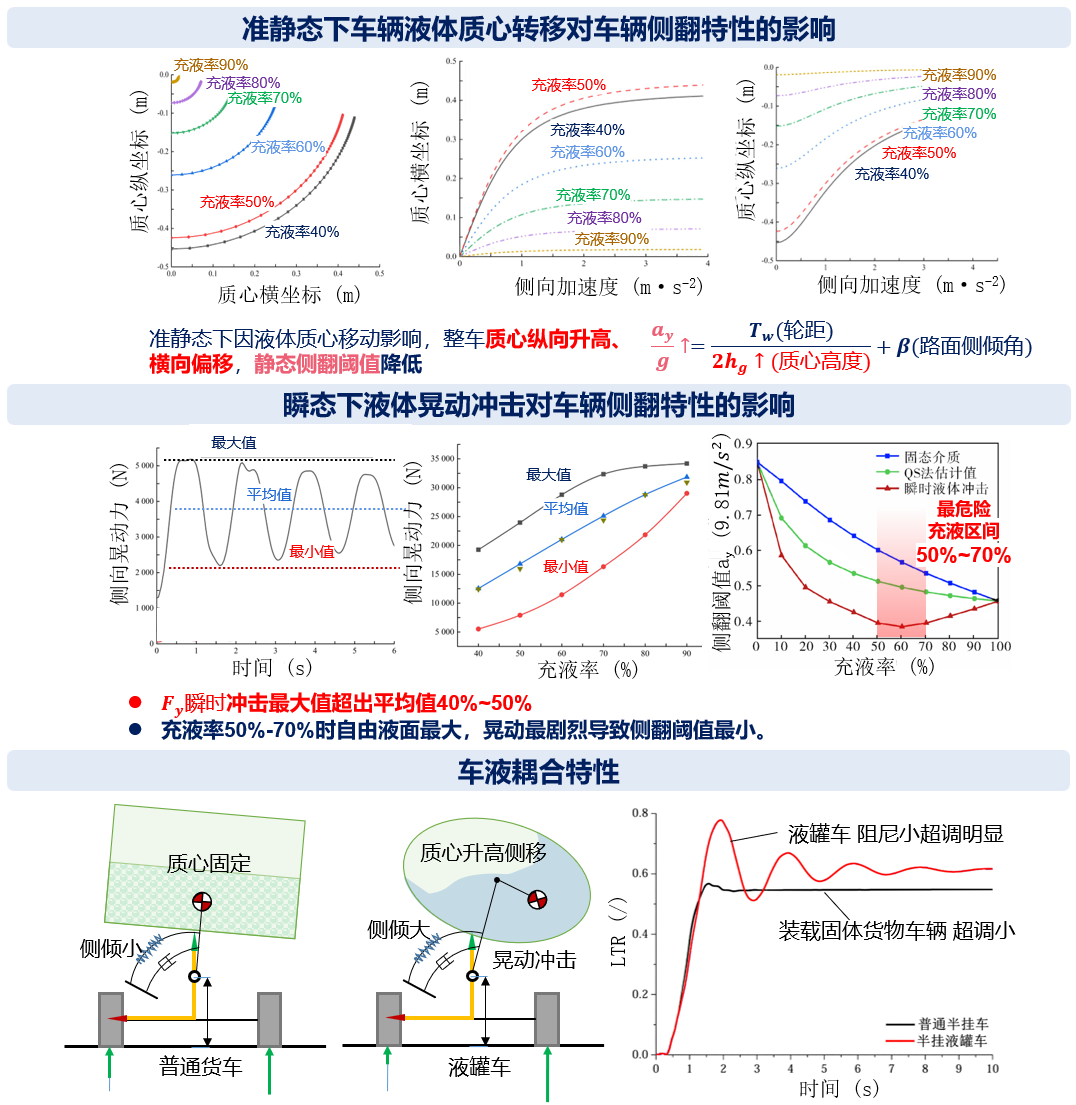
\includegraphics[width=1.0\linewidth]{fig/chap1/two_factors.png}
        \caption[车液耦合机理说明]{车液耦合机理说明\cite{maohaijian2021fsi,huangyang2017impact,wangqiongyao2017sloshing,wanying2020antirolover}}
        \label{fig:vehicle_liquid_couple_mechanism}
      \end{figure}

      相较于固体载荷车辆中“载荷增加导致侧翻阈值单调下降”的一般规律，液罐车在部分充液条件下通常表现出更复杂的非单调特征。现有研究普遍表明，车辆侧翻风险随充液率变化往往呈现“先降低后回升”的趋势，中等充液率常对应更不利工况，尤其在\SIrange{50}{70}{\percent}附近更易出现显著晃动冲击。这表明，除总质量与质心高度变化外，自由液面长度、液体惯性分量及瞬态冲击效应也是决定液罐车侧倾稳定性的关键因素\cite{maohaijian2021fsi,wangxiaorun2022lateralacc,yuzhixin2018mpc,xuxiaomei2020lanechange,lijie2020carliquid}。代表性研究进一步指出，中等充液率下液体横向冲击更强、侧向力波动更显著，而在高充液率条件下，自由液面受限，晃动幅值与波动程度通常有所抑制\cite{wangxiaorun2022lateralacc,wangqiongyao2017sloshing}。


      从影响因素看，现有研究普遍认为液体晃动强度主要受液体质心高度、自由液面长度以及外部激励特性共同影响。质心越高，液体重力引起的平均侧倾力矩越大；自由液面越长，液体横向迁移与冲击越剧烈，系统响应中的高阶分量也越明显；而激励幅值与频率则影响主导响应模态及能量分布，从而改变晃动峰值及衰减特性\cite{chenyibao2016crosssection,wangqiongyao2017sloshing}。

      因此，车--液耦合对液罐车侧向动力学的影响可概括为三个方面：一是准静态质心迁移增大等效侧倾力矩，使响应幅值上升；二是瞬态晃动冲击带来附加侧向力与侧倾力矩，使系统更易出现峰值放大和超调；三是液体系统阻尼有限，导致振荡衰减较慢、危险状态持续时间延长。上述特性共同解释了液罐车在中等充液率和强横向激励条件下更易发生侧倾失稳，也表明后续建模需要在关键模态可解释性与实时性之间进行权衡。

    \subsubsection{液体晃动建模研究现状}
    \label{subsub:liquid_shaking_modeling}

      液体晃动建模最早主要面向飞行器燃料箱、船舶液舱和车辆油箱等场景，近年来逐步扩展到液罐车晃动与侧倾稳定性研究。现有方法大体可归纳为四类：准静态模型法、机械等效力学模型法、液体晃动动力学模型法和实验研究法\cite{jiaxinhong2022review}，如图~\ref{fig:liquid_modeling_methods}所示。四类方法分别对应稳态规律分析、低维动态近似、高精度流动求解和模型验证等不同目标。

      \begin{figure}
        \centering
        \subcaptionbox{准静态模型法\cite{huangyang2017impact}\label{fig:liquid_model_qs}}
          {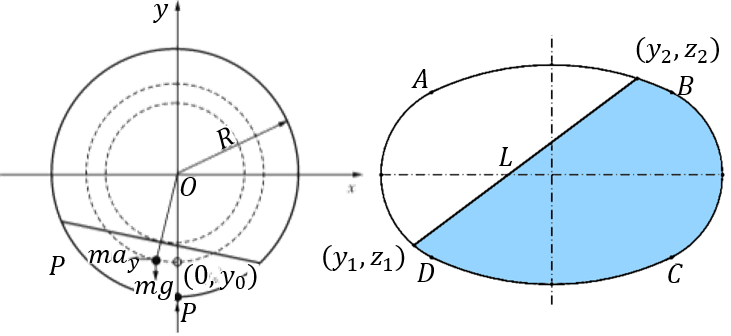
\includegraphics[width=0.48\linewidth]{fig/chap1/quasi_static.png}}
        \subcaptionbox{液体晃动动力学模型法\cite{maohaijian2021fsi,yuzhixin2018mpc}\label{fig:liquid_model_cfd}}
          {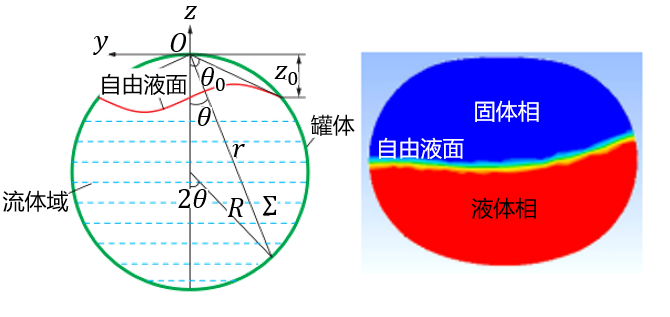
\includegraphics[width=0.48\linewidth]{fig/chap1/fluid_dynamic_model.png}}
        \subcaptionbox{实验研究法\cite{wangxiaorun2022lateralacc,wanying2020antirolover}\label{fig:liquid_model_experiment}}
          {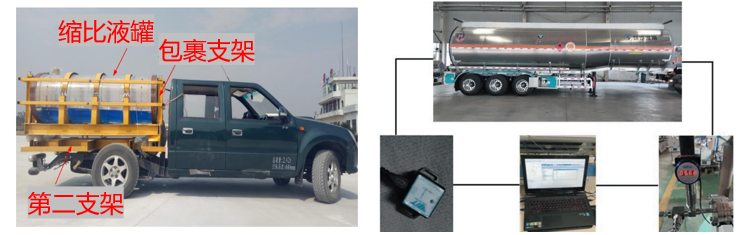
\includegraphics[width=0.48\linewidth]{fig/chap1/experiment_method.png}}
        \subcaptionbox{机械等效力学模型法\cite{yuzhixin2019optimalcontrol,zhaoweiqiang2018equivalent,zhaoweiqiang2019semitrailer}\label{fig:liquid_model_equivalent_model}}
          {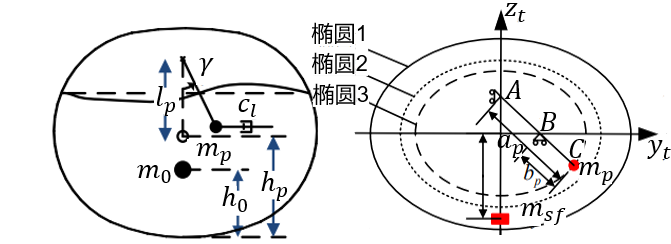
\includegraphics[width=0.48\linewidth]{fig/chap1/equivalent_model.png}}
        \caption{液体晃动建模方法}
        \label{fig:liquid_modeling_methods}
      \end{figure}

      \emph{准静态模型法（QS）}基于自由液面形态、液体质心位置和静力平衡关系描述平均晃动力与侧倾力矩，形式简单、物理意义明确，适合分析充液率、截面形状等因素对稳态侧倾特性的影响\cite{huangyang2017impact,helieyun2020quasistatic}。但该方法忽略瞬态晃动冲击和相位滞后，对变道、蛇形等非稳态工况的适用性有限。

      \emph{机械等效力学模型法}通过单摆、双摆、弹簧--质量--阻尼或椭圆规摆等低维结构逼近液体晃动产生的等效力和力矩\cite{salem2000rollover,yangxiujian2018multimass,wuxiangji2018sloshingmodel,Komasa2023observing,KomasaQi2025AntiRollover_TITS}。其优势在于计算效率高、易于嵌入规划与控制，是当前最适合在线应用的一类方法。其不足在于表达能力受等效结构限制，通常只能覆盖主导模态，对高阶晃动、水跃飞溅及横纵向耦合流动的描述仍不充分。

      \begin{figure}
        \centering
        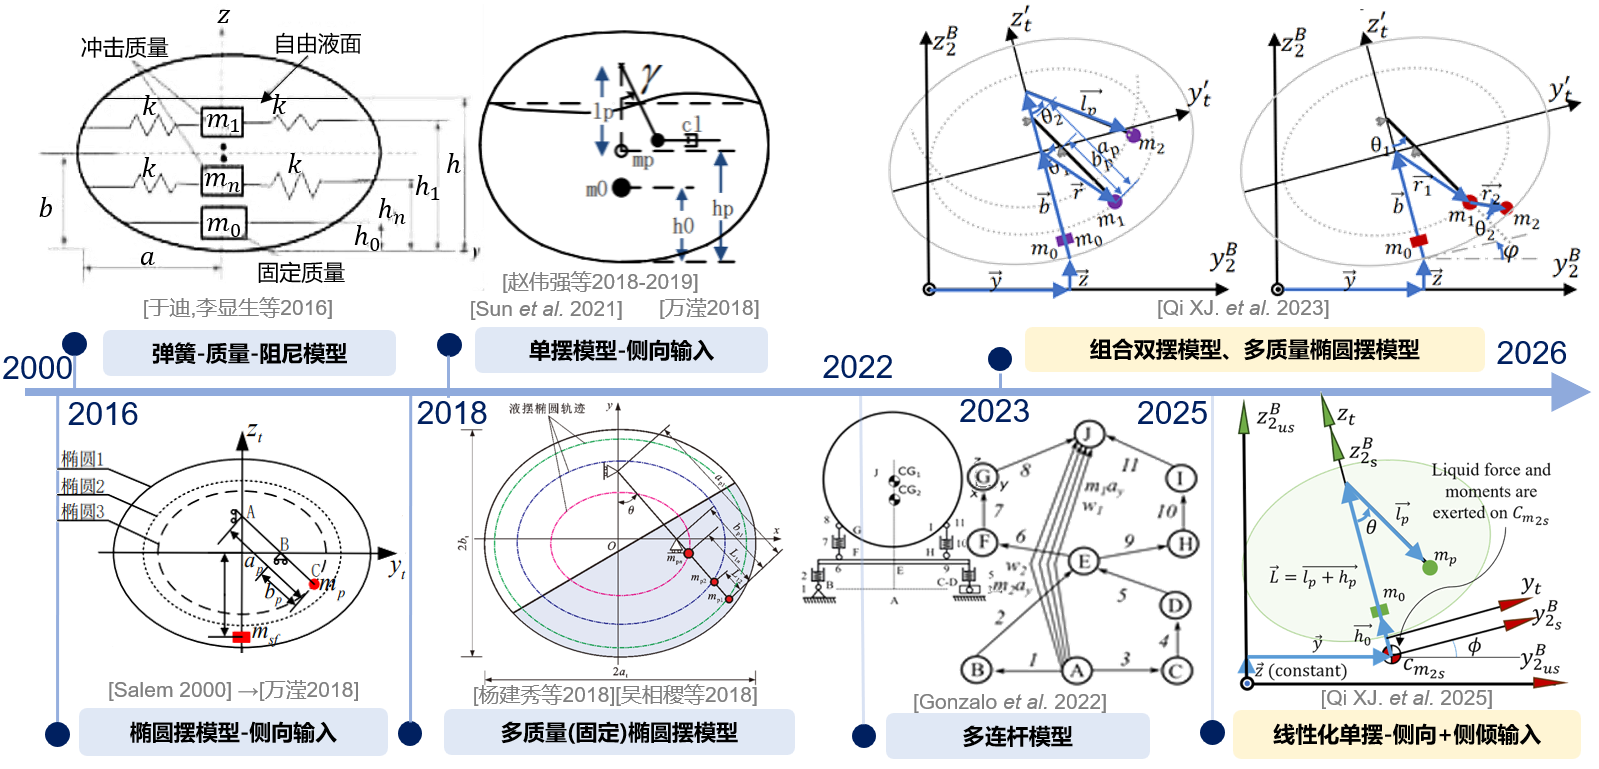
\includegraphics[width=1.0\linewidth]{fig/chap1/machenical.png}
        \caption{液体晃动机械等效模型发展}
        \label{fig:machenical}
      \end{figure}

      \emph{液体晃动动力学模型法}直接基于流体动力学方程描述液体运动，典型包括线性晃动理论和CFD方法。该类方法能够较完整地刻画自由液面演化及强非线性流动，精度高，适合机理分析、高精度基准构建和离线标定\cite{maohaijian2021fsi,yuzhixin2018mpc}。但其建模与求解代价较大，通常难以满足实时规划与控制需求。

      \emph{实验研究法}通过实车、缩比模型或液舱台架直接观测晃动行为和车辆响应，是模型校核与控制验证的重要手段\cite{wangxiaorun2022lateralacc,wanying2020antirolover}。但受安全性、成本和可重复性限制，尤其在危化品场景下难以大规模开展，因此更多承担验证作用，而难以替代建模本身。

      总体来看，现有研究已经形成“准静态方法揭示平均规律、机械等效模型服务实时应用、流体动力学模型提供高精度基准、实验方法承担验证闭环”的基本格局。其中，机械等效模型最适合车辆规划与控制，但现有模型多集中于二维主导晃动，对横摆、俯仰以及纵向加减速诱导的横纵向流动耦合考虑不足。对于液罐车防侧翻问题，后续建模的关键不在于单纯提高复杂度，而在于在保证实时性的前提下保留对侧倾失稳最关键的液动模态。

    \subsubsection{液罐车动力学建模研究现状}
    \label{subsub:vehicle_dynamics}

      在规划与控制中引入液罐车动力学约束，首先需要建立可计算的车--液耦合动力学模型。受工程实时性要求限制，现有研究通常采用“简化车辆模型 + 液体晃动模型” 的建模路线，即以低自由度车辆横向/横摆模型为骨架，并与准静态模型、机械等效模型或流体动力学模型耦合，形成可用于分析、规划与控制的低阶模型\cite{yudi2019rollstability,wanying2020antirolover,yuzhixin2018mpc}。

      对整体式液罐车而言，车辆部分多采用自行车模型、3DOF平面模型或引入侧倾自由度的4DOF模型，以兼顾横向运动描述与侧翻风险表征\cite{renyuanyuan2020precisemodel,wanying2020antirolover,yudi2019rollstability}。其中，3DOF模型适合描述纵向、侧向和横摆运动，4DOF模型则进一步增强了对侧倾响应的刻画能力；与之耦合的液体模型通常采用单摆、椭圆规摆等机械等效形式，以满足计算效率要求\cite{renyuanyuan2020precisemodel,wanying2020antirolover}。总体上，这类模型能够较好支撑液罐车与固体载荷车辆的动力学差异分析，以及抑晃和防侧翻控制器设计\cite{renyuanyuan2020precisemodel,wanying2020antirolover}。

      对半挂液罐车而言，由于牵引车与挂车之间存在铰接耦合，系统动力学维度更高，建模时通常需要围绕研究目标进一步简化。现有研究常采用牵引车与挂车平面运动模型描述基本操纵特性，例如制动分析中常见牵引车纵向、侧向、横摆与挂车横摆组成的4DOF模型\cite{heren2016braking}；在防侧翻研究中，则更多采用包含牵引车侧倾和挂车侧倾的5DOF模型，以增强对侧倾稳定性的表达\cite{zongchangfu2014identification,niezhigen2015heavyduty}。在此基础上，再与基于势流理论、单摆或椭圆规摆的液体模型耦合，可形成适用于半挂液罐车分析与控制设计的低阶车--液耦合模型\cite{yuzhixin2018mpc,yuzhixin2019optimalcontrol}。因此，“半挂车简化动力学模型 + 可计算液体模型”已成为半挂液罐车工程建模的主流思路\cite{yuzhixin2018mpc,zongchangfu2014identification}。

      除模型结构外，参数辨识也是决定模型可用性的关键环节。现有研究通常以高精度仿真或实验结果为参照，通过遗传算法、粒子群等优化方法最小化低阶模型与参考模型之间的输出误差，从而辨识液体等效参数和部分车辆参数\cite{wanying2020antirolover,yudi2016nonfull,zongchangfu2014identification,niezhigen2015heavyduty}。其中，液体部分的辨识重点在于使等效模型逼近CFD或实验得到的侧向力、侧倾力矩等关键输出\cite{wanying2020antirolover,yudi2016nonfull}；车辆部分则常需结合多工况辨识和参数插值，以适应运行状态变化\cite{zongchangfu2014identification,niezhigen2015heavyduty}。

      总体来看，现有液罐车动力学建模已形成以低自由度车辆模型耦合可实时液体模型的基本框架：整体式液罐车多采用3--4DOF车辆模型，半挂液罐车多采用约5DOF的简化模型，并配合单摆、椭圆规摆等机械等效液体模型，在精度与实时性之间取得折中\cite{renyuanyuan2020precisemodel,wanying2020antirolover,yuzhixin2018mpc,yuzhixin2019optimalcontrol}。但现有模型仍普遍存在横纵向耦合不足、输出模态有限，以及对复杂交通工况和强非线性液体响应适应性不足等问题，这也说明后续研究需要进一步面向预测性规划与鲁棒控制任务，提升模型对关键失稳模态的表达能力。

  \subsection{液罐车防侧翻主动安全措施研究现状}
    通过液罐车自身的改进解决其侧倾稳定性差问题的思路有两大类，一类是以改进车辆自身性能的被动措施；另一类是从控制入手的主动安全措施。被动安全措施已在罐体形状优化\cite{chenyibao2016crosssection,quhuijun2017calculation,yudi2016nonfull,yudi2019rollstability,lixiansheng2015ga}、防浪结构设计\cite{hanyoubin2019vof,moreno2022davies,liukui2009braking,liukui2009steering}和自由液面抑制\cite{wangqiongyao2017sloshing}等方面形成较为系统的研究与工程基础，能够在一定程度上降低液体晃动强度并改善车辆侧倾稳定性。但这类方法主要作用于车辆和罐体本体，其效果受整车布置、制造成本、轻量化要求以及检修维护条件限制，难以持续覆盖道路几何突变、周车干扰、驾驶操作失误等外部诱因所导致的动态风险。因此，仅依赖被动措施仍难以充分应对复杂交通环境下的侧翻问题，仍需结合主动风险预测、预防性规划与控制干预，形成与被动措施互补的分层安全体系。

    面向液罐车的主动防侧翻方法总体可归纳为两条互补路径：\emph{防侧翻运动规划}与\emph{防侧翻控制}。前者通过在决策与轨迹层提前约束侧向激励、侧倾响应及其演化过程，从源头降低车辆进入危险状态的概率，更偏向“预防”；后者则在车辆已处于高侧翻风险状态时，通过执行器施加控制作用抑制侧倾失稳，更偏向“救车”。考虑本文对象为半挂式液罐车，其防侧翻问题同时受到半挂结构、液体晃动耦合及自动驾驶执行条件的共同影响，因而有必要分别从防侧翻运动规划与防侧翻控制两方面进行综述。

    \subsubsection{防侧翻运动规划研究现状}

      防侧翻运动规划的核心是在轨迹生成阶段显式约束可能诱发侧翻的横向激励与姿态响应，因此首先需要合理刻画侧翻风险。现有研究常用指标大致可分为三类：一类是以SSF、DSF为代表的稳定性判据，适合描述车辆几何与动力学层面的稳定裕度\cite{huston2014ssf,jin2007critical,heyuancha0_2010factor}；一类是以LTR及其变体为代表的载荷转移指标，能够较直接反映车轮接地载荷变化，是当前防侧翻规划与控制中最常用的动态风险指标\cite{zhang2016pulsed,zhao2019hinfty,jin2021heavytruck}；另一类是TTR、ZMP及多参数联合指标，更适用于风险预警、触发逻辑或综合安全评估\cite{wanying2020antirolover,zeng2017bpnn,jinliqiang2017yujing,jin2016tripped,jin2019triaxle,imine2015switched}。总体而言，LTR兼具物理可解释性和动态敏感性，在防侧翻运动规划中应用最为广泛。

      在此基础上，现有防侧翻规划通常是在通用轨迹规划框架中引入侧倾动力学约束或风险代价，以限制侧向加速度、横摆响应和载荷转移峰值。按方法形式划分，相关研究大体可归纳为搜索、采样、几何参数化、优化和学习五类。搜索类方法如A*、混合A*、动态规划（Dynamic Programming, DP）和格点规划器（Lattice Planner）等\cite{likhachev2009planning,kurzer2016hybrida,dong2023ecocruising,werling2010frenet}，具有较好的可行性搜索能力，但受限于状态离散化，较难细致表达连续动力学约束和风险演化；采样类方法如概率路图法（Probabilistic Roadmap, PRM）、快速拓展随机树（Rapidly-exploring Random Tree, RRT）及其变体\cite{kuwata2009realtime,karaman2011sampling,klemm2015rrtconnect,fan2024birrt}，适合复杂环境中的可行域探索，但结果一致性和约束稳定性相对不足；几何参数化方法基于回旋曲线、贝塞尔曲线、B样条等直接构造连续轨迹\cite{brezak2014clothoids,rastelli2014continuouscurvature,phanhuu2021bsplines,gotte2018splinebased,hegedus2020realtime}，计算效率较高，但对复杂约束和多目标权衡的表达能力有限。相比之下，优化方法能够将避障约束、轨迹平滑性与载荷转移率（Load Transfer Ratio, LTR）、侧翻时间（Time to Rollover, TTR）等防侧翻指标统一纳入目标函数或约束条件，因此已成为防侧翻规划研究的主要方向\cite{rasekhipour2017pfmpc,jin2021heavytruck,cheng2019longitudinal,li2019rollover,dong2023ecocruising}；学习方法则多以强化学习及安全强化学习（Safe Reinforcement Learning, Safe RL）为基础，试图在复杂交互环境中直接学习兼顾安全与效率的行为策略\cite{wu2024rlsurvey,zhang2023intersectionrl,irshayyid2024highwayrl,zhang2024saferl_tits,gu2024saferl_tpami,garcia2015saferl}，但其性能仍高度依赖场景覆盖、奖励设计和安全约束构造。

      对半挂式液罐车而言，防侧翻规划比普通车辆更为复杂。半挂结构引入牵引车--挂车铰接耦合，使规划过程除满足牵引车本体避障外，还需兼顾挂车轨迹约束、铰接角稳定性和防折叠要求\cite{zongchangfu2014identification,niezhigen2015heavyduty}；液体晃动进一步与横摆、侧倾和路径变化相互耦合，使规划问题由一般动力学可行性问题演化为受强安全约束主导的耦合规划问题。因此，液罐车防侧翻规划不仅要控制轨迹几何形状，还要限制由路径变化激发的侧倾风险累积。现有半挂车规划研究为此提供了一定基础。低速场景研究多集中于自动泊车和狭小空间避障，通常基于半挂车运动学模型，将搜索、采样、优化或强化学习方法用于牵引车轨迹生成，并通过铰接角和挂车避障约束保证整体可行性\cite{wangyuanmin2024,chenchao2023,jiasenchao2023}。高速场景研究则更关注牵引车与挂车协同跟踪、高速换道与稳定性保持，常通过LQR、ADP、优化方法或分层控制框架降低铰接角误差、挂车跟踪误差及峰值LTR\cite{lisixu2021,caoliling2024,zhangfawang2025,songguanghao2023,wanghongchang2023}。但这些研究大多面向一般半挂车，重点仍在避障、泊车或高速跟踪，对液体晃动与侧翻风险的考虑相对有限。

      总体来看，现有研究已经形成较丰富的防侧翻风险指标体系和通用规划方法，也为半挂车轨迹生成与协同跟踪提供了基础；但公开文献中仍缺少真正面向半挂式液罐车的防侧翻运动规划方法。具体而言，普通车辆防侧翻规划通常未显式考虑牵挂结构与液体晃动耦合，而现有半挂车规划研究又多未将液体动力学和强侧翻约束纳入统一规划框架。因此，面向自动驾驶场景构建兼顾半挂结构、液体晃动与侧翻风险约束的防侧翻运动规划方法，仍是有待突破的关键问题。

    \subsubsection{防侧翻控制研究现状}

      与防侧翻运动规划侧重从源头降低风险不同，防侧翻控制更强调在车辆接近危险边界或已进入危险状态时，通过执行器快速干预侧倾动态。现有车辆防侧翻控制方法主要包括主动悬架、差动制动、分布式驱动、转向控制及其组合形式\cite{xu2011rollover,liang2022multiagent}。其中，主动悬架通过调节左右悬架支撑力直接作用于侧倾自由度，控制效果最直接，但硬件复杂度和能耗成本较高\cite{xiao2020rollsuspension}；差动制动依托左右轮制动力差产生附加横摆力矩，工程实现基础较好，但对侧倾的作用路径较为间接\cite{carlson1981two}；分布式驱动可进一步扩大可用横摆力矩，但通常依赖特殊驱动结构，应用范围有限\cite{zilin2023integrated}；转向控制则通过改变车辆路径和横向激励主动抑制侧翻风险，在极限工况下通常具有更强的翻车避免潜力，但对执行器能力和控制设计要求更高\cite{shao2023vhrobustmpc}。

      \begin{figure}
        \centering
        \subcaptionbox{主动悬架\label{fig:active_suspension}}
          {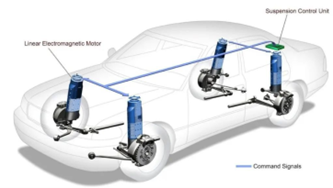
\includegraphics[width=0.40\linewidth]{fig/chap1/active_suspension.png}}
        \subcaptionbox{转向控制(前轮和/或后轮)\label{fig:active_steering}}
          {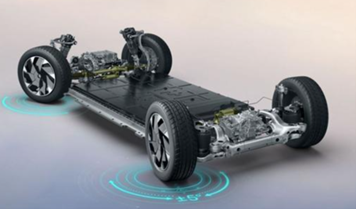
\includegraphics[width=0.40\linewidth]{fig/chap1/active_steering.png}}
        \vspace{0.2cm}
        \subcaptionbox{差动制动\label{fig:diff_braking}}
          {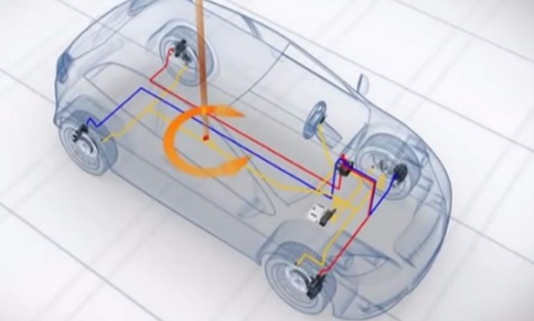
\includegraphics[width=0.40\linewidth]{fig/chap1/diff_braking.png}}
        \subcaptionbox{分布式驱动\label{fig:distributed_driving}}
          {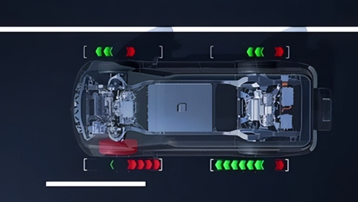
\includegraphics[width=0.40\linewidth]{fig/chap1/dist_driving.png}}
        \caption{现有车辆防侧翻控制方法}
        \label{fig:anti_rollover_methods}
      \end{figure}

      对液罐车而言，防侧翻控制仍属于相对小众的研究方向，现有工作总体上主要面向人工驾驶条件下的主动安全辅助。受车载硬件条件和工程可实施性限制，相关研究主要集中于差动制动、转向控制及其协同形式，而主动悬架和分布式驱动在液罐车领域中的研究和应用相对较少\cite{zhaoweiqiang2018equivalent,yuzhixin2018mpc,weixing2023_antirollover}。在建模层面，现有研究通常采用等效摆模型或势流模型描述液体晃动，并与车辆横向动力学模型耦合\cite{zhaoweiqiang2018equivalent,yuzhixin2018mpc,yuzhixin2019optimalcontrol,wanying2020antirolover}；在控制层面，则主要采用PID及模糊PID、LQR、MPC、无模型自适应控制和$H_\infty$控制等方法\cite{huyun2019mfac,luoyugong2019sbw,tangzeyue2023mpcmfac,fengzengxi2021mfacpso,zhao2019hinfty}。从研究演进看，早期工作多采用“液体机械等效模型 + 差动制动救车”的基本范式\cite{zhaoweiqiang2018equivalent,zhaoweiqiang2019semitrailer}，随后逐步发展为将势流或等效摆液体模型与半挂车动力学耦合，并结合MPC、LQR等方法实现差动制动与转向控制协同\cite{yuzhixin2018mpc,yuzhixin2019optimalcontrol,Reviewer2_SunWencai2022,wanying2020antirolover}。与此同时，高精度CFD仿真也开始用于液体动力学分析及控制方法验证，从而提升了液体建模和验证的可信度\cite{lijie2020carliquid,wanying2020antirolover}。从控制效果看，现有研究普遍表明，差动制动工程可实施性较好，但由于其主要通过附加横摆力矩间接影响侧倾动态，控制能力存在上限\cite{liutianfeng2024heterogeneous}；相比之下，转向控制通过直接改变车辆路径和横向激励，通常在稳定时间、超调抑制和峰值LTR降低等方面表现更优\cite{MFAC_LiXiansheng2021,zhengxuelian2019mfacpatent}。近年来，随着自动驾驶液罐车研究的推进，部分工作开始尝试将防侧翻控制由单一临险干预扩展到路径跟踪与防侧翻协调控制，以实现“常态运行 + 临险补偿”的多模态安全控制\cite{weixing2023_antirollover}，但切换标准及过渡手段仍需进一步研究。

      总体来看，现有液罐车防侧翻控制研究已在执行器选择、液体建模、控制方法和验证手段等方面取得一定进展，但总体上仍以紧急救车和事后抑制为主，对自动驾驶条件下更重要的预防性安全保障关注不足。现有方法普遍建立在横纵向解耦、液体模型简化和局部控制补偿基础上，对液体横纵向耦合流动、规划与控制协同以及复杂场景验证闭环的考虑仍不充分。因此，面向半挂式液罐车，有必要进一步将转向控制、差动制动等执行手段与防侧翻运动规划协同设计，形成“提前避险 + 临险兜底”的主动安全控制框架。


  \subsection{车云协同预测性决策与规划研究现状}

    云端预测性行为决策与运动规划是在单车自动驾驶决策与规划的基础上发展而来的，相对于单车方案，云端预测性的决策和规划更加考虑了云端的全局感知、并行算力与协同优化优势，对单车所触及不到的长时域规律进行解析，并给出更具指导性的建议。

    \subsubsection{单车智能行为决策及其向云端的拓展}
      \label{subsub:autonomous_decision}

      尽管云端与车端在可用信息量、更新频率与规划颗粒度上存在差异，其决策与规划的基本范式是相通的：在不确定、多主体交互的交通环境中，生成既安全又高效且可执行的行为与轨迹。因此，较为成熟的单车智能行为决策为云端预测性决策提供了重要参考。行为决策自始至终试图解决的核心问题只有一个：\emph{如何处理自车与周围交通参与者之间的交互}，如图~\ref{fig:pred_dec_int}所示。

      自DARPA自动驾驶挑战赛以来，感知--预测--决策--规划--控制的模块化流程被沿用多年\cite{ferguson2008urban,urmson2008boss,leonard2008perception,kammel2008annieway,vonhundelshausen2008tentacles,montemerlo2008junior,thrun2006stanley}，但该流程隐藏了一个关键逻辑矛盾：若先对周车进行预测再据此决策，则预测结果默认与自车决策无关；而实际交通中周车行为往往会对自车动作产生反应，预测应当随自车候选决策而变化。由此，传统“先预测后决策”的串行结构在多车交互场景下容易出现保守、迟滞或不稳定等问题。为修正上述矛盾，近年来模块化路线的一个共同趋势是\emph{预测--决策一体化}。
      
      现有模块化方法大体可按交互处理方式划分为显式交互、隐式交互及综合式交互三类。\emph{显式交互}以自车候选策略/意图划分场景，在每个候选行为下预测周车反应，并对不同候选行为的长期收益与风险进行比较，典型代表为多策略决策方法（Multi-Policy Decision Method, MPDM）；\emph{隐式交互}侧重对周车意图/不确定性构造多个可能情景，并在情景集合上评估自车应对策略，典型代表包括防御性规划（Contingency Planning）\cite{salvado2016contingency}与博弈论方法；\emph{综合式交互}将显式交互与隐式交互思想融合，并常与风险度量、礼貌性或协同性等机制结合\cite{KomasaQi2026Appendix}。
  
      端到端方案则进一步通过学习从环境表征到行为/轨迹的可微分联合映射，在训练阶段将预测、决策与规划的耦合显式纳入优化目标，从而缓解传统“先预测后决策”带来的交互一致性问题。常见实现包括基于模仿学习的端到端轨迹生成、基于强化学习的交互策略学习，以及以扩散/生成模型为代表的多模态规划生成等。端到端方法中较早发展起来的两段式端到端方法融合预测--决策--规划三者，近年来涌现的一段式端到端则将感知--规划的闭环打通，其中VLA方案则将感知--控制全链路打通\cite{KomasaQi2026Appendix}。

      \begin{figure}
        \centering
        \subcaptionbox{预测决策一体化\label{fig:pred_dec_int1}}
          {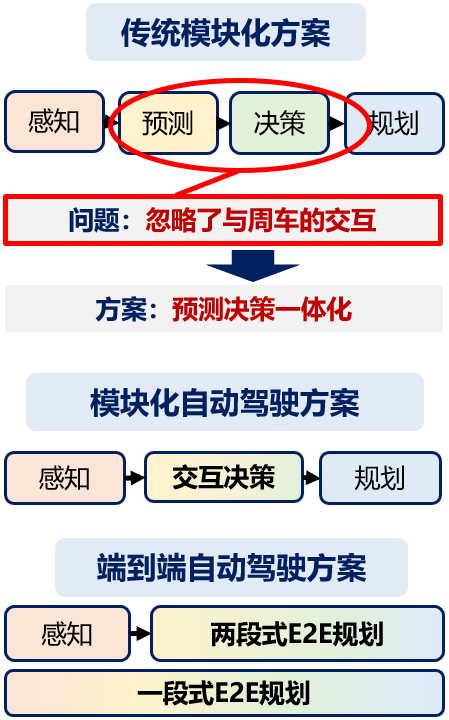
\includegraphics[width=0.32\linewidth]{fig/chap1/pred_dec_int1.png}}
        \subcaptionbox{交互决策大尺度拓展\label{fig:pred_dec_int2}}
          {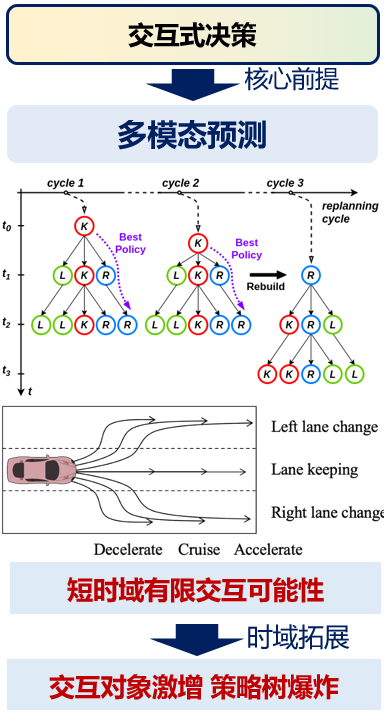
\includegraphics[width=0.275\linewidth]{fig/chap1/pred_dec_int2.png}}
        \subcaptionbox{两段式端到端大尺度拓展\label{fig:pred_dec_int3}}
          {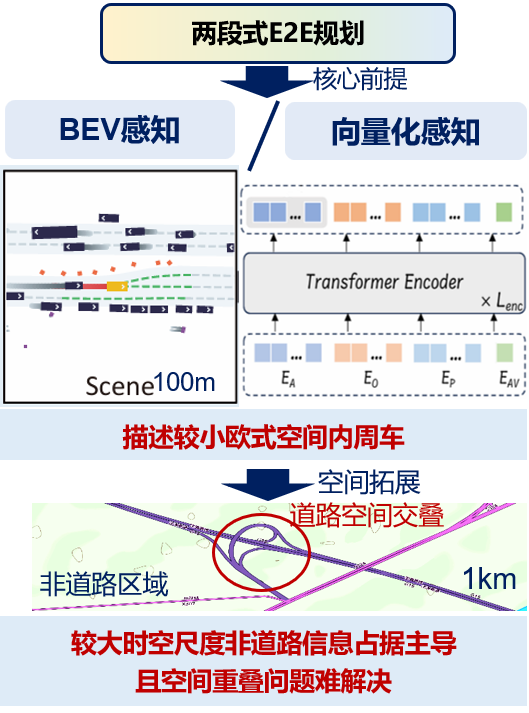
\includegraphics[width=0.38\linewidth]{fig/chap1/pred_dec_int3.png}}
        \caption{预测决策一体化思想及其向大时空尺度的拓展}
        \label{fig:pred_dec_int}
      \end{figure}

      对云端预测性行为决策而言，预测决策一体化的核心思想同样适用，但现有单车方案向云端长时域大空间尺度的拓展存在挑战。模块化方案的交互式决策需具备多模态周车预测能力从而据其构建自车行为树，但随着云端时域与空间尺度的增加，周车行为树的规模将呈指数级增长，导致计算复杂度过高，且预测结果无法穷尽所有可能，即每次交互将忽略大量小概率事件，而这在长时域多次交互后将导致不确定性传播的严重失真；由于车云通信时延，端到端方案在云端通常采用两段式，其依赖的BEV感知特征或向量化感知适合描述小欧式空间内周车，在面对大时空尺度拓展时则包含大量无用非道路语义向量子空间，导致表征与计算效率低下。

      综上，单车自动驾驶的行为决策普遍通过预测--决策耦合的方式高效建模自车与周车的短期交互以规避先预测后决策的逻辑谬误，云端预测决策一体化势在必行。然而，现有适用于单车的交互建模方式难以拓展到需要考虑较大时空尺度的云端，亟需适用于云端的反映交互不确定性在长时域扩散的交互建模方法。

    \subsubsection{云控预测性决策与规划研究现状}
      \label{subsub:cloud_control}

      相较于单车自动驾驶主要依赖本车局部感知、短时域预测和有限车载算力完成决策与规划，车路云一体化系统可借助路侧、边缘侧或云端的广域感知与并行计算能力，在车端实时闭环之外提供更长时域的预测性决策与规划支持，从而弥补单车在全局可观测性、预测范围和计算资源上的不足\cite{Huang2025V2X}。

      从功能分配方式看，现有云控预测性决策与规划研究大体可归纳为三类：车端决策辅助、车云分层控制和云端全局/集中控制\cite{Huang2025V2X}。其中，车端决策辅助仍以车端为决策主体，仅利用V2X信息增强环境理解、行为预测和本地规划\cite{UniV2X2024,UniMM_V2X2025,V2X_VLM2025}；该类方法实现门槛较低、易于与现有单车系统结合，但并未根本改变“决策主要在车端完成”的结构，因此对车端算力压力和全局协同能力的改善有限。云端全局/集中控制则进一步将决策重心转移至路侧、边缘侧或云端，由基础设施在交叉口、匝道或更大路网尺度统一组织多车行为\cite{Kherroubi2024AUTODRAITEC,Lu2024EdgeComputing,Typaldos2025Cooperative,Yang2025CloudBased,Wang2025Cooperative,shijia2024rampcloud}；该类方法最能发挥广域感知和全局优化优势，但对通信可靠性、渗透率和基础设施部署条件要求较高，在现实交通环境下应用边界较强。相比之下，车云分层控制强调“云端长时域引导、车端短时域闭环”，由云端负责低频、预测性和全局性决策，车端负责高频、强安全约束下的轨迹生成与稳定控制\cite{Gao2025V2X,hans2024,chenqien2023cpccbus,lishuyan2022pccheavytrucks,wangluyao2024cloudpacc,wangzhou2023hierarchical,meirun2023platoon,jiangyu2023lc}。这类方法既能利用云端扩展预测时域和协同范围，又保留了车端安全闭环，因此更符合当前低渗透率、通信资源受限条件下的工程实现需求。需要指出的是，车云协同的关键并不只是“云端是否更优”，而在于云端建议能否在通信时延、丢包和链路波动条件下被车端稳定吸收并保持安全闭环\cite{xionglu2024_CVIS_survay,xuqing2021unreliable,wang2021platoonmpc}。因此，现有车云分层方法通常还需要结合时间触发、事件触发、局部重规划和降级执行等机制，以处理通信不确定性并维持系统鲁棒性\cite{hans2024,wang2021platoonmpc}。

      从应用目标看，现有云控预测性决策与规划研究主要面向一般自动驾驶场景下的安全、节能和通行效率优化，典型任务包括换道辅助、速度规划、队列组织、匝道合流和路口冲突协调\cite{chenqien2023cpccbus,wangzhou2023hierarchical,meirun2023platoon,Typaldos2025Cooperative,Yang2025CloudBased}。这些研究为云端参与行为决策和长时域规划提供了方法基础，但其协同对象多为普通车辆，关注点也主要是交通效率、能耗或一般安全性提升。对于液罐车而言，侧翻风险不仅受道路与周车行为影响，还与液体晃动、车辆侧倾及半挂结构耦合密切相关，因此云控问题不再只是一般意义上的行为优化，而是面向强安全约束和强动力学耦合条件下的预测性风险规避问题。

      目前车路云协同决策与规划已形成由“车端决策辅助—车云分层控制—云端全局/集中控制”构成的连续谱系。其中，车端决策辅助易于部署，但协同深度有限；云端全局/集中控制优化潜力最大，但对外部条件依赖最强；车云分层控制则在协同收益与工程可行性之间取得了较好平衡，更适合作为当前阶段车云协同液罐车防侧翻问题的基本架构。尽管如此，现有研究仍主要面向普通自动驾驶任务，尚缺少针对液罐车防侧翻这一强安全约束问题的系统设计，尤其缺少对云端预测性决策、车端防侧翻运动规划与稳定控制之间协同机制的统一刻画。因此，如何在低渗透率和通信不可靠条件下明确云端与车端的功能边界、信息接口、触发机制与降级关系，进而构建可降级、可验证、可持续演进的车云协同防侧翻决策与规划框架，仍是亟待解决的关键问题。

  \subsection{车云协同体系架构构建方法研究现状}

    前述研究表明，液罐车防侧翻问题已在车--液耦合建模、车端防侧翻控制和车云协同预测性决策等方面形成了一定技术积累，但现有研究大多聚焦局部机理、单项算法或单一场景优化，尚缺少一种能够将需求、能力、功能、逻辑、资源与验证机制统一映射的体系架构构建方法。对于车云协同液罐车防侧翻问题，仅从规划、控制或通信等单一层面分别展开研究，难以回答云端与车端如何分工、系统边界与接口定义、异常行为挖掘及应对方式、以及架构如何验证等更基础的体系问题。

    在这一背景下，车路云一体化为智能车辆系统提供了新的工程组织方式，其核心在于将车辆、路侧基础设施、云端计算资源和平台服务进行系统级连接，以支撑广域感知、协同决策与闭环控制\cite{likeqiang2020cloudcontrol,likeqiang2020principles,icv2023whiteroadcloud,ran2023vrc,guo2023greeniov}。在系统抽象层面，该类对象通常可归纳为智能汽车信息物理系统（Intelligent Vehicle Cyber-Physical System, IVCPS）。因此，车路云一体化更适合作为工程建设范式，而IVCPS则是其对应的系统形态表达；本文研究的车云协同液罐车防侧翻（Cloud-based Collaborative Tank Truck Rollover Prevention, CT2ROP）可视为IVCPS中一个面向安全的典型场景任务。

    围绕此类复杂交通系统，国内外已形成若干代表性参考架构。例如，美国交通部发布的网联车辆参考实施架构（Connected Vehicle Reference Implementation Architecture, CVRIA）和协同式智能交通系统参考架构（Architecture Reference for Cooperative and Intelligent Transportation, ARC-IT）从企业、功能、物理、通信和服务等多个视角描述网联交通系统组成与交互关系\cite{hejazi2022iottov2x,usdot2024arcit93}；欧盟C-MobILE项目面向协同式智能交通系统（Cooperative Intelligent Transport Systems, C-ITS），从上下文、功能、通信、应用和信息等视角开展架构描述，并探索了基于SysML的建模方法\cite{cmobile2024project,lu2018citsdeployment,ferrandez2018cmobilecase}；国内则已形成智能汽车信息物理系统参考架构1.0/2.0、ICV-7S框架以及车路云一体化系统云控基础平台功能场景参考架构等成果\cite{caicv2019cpsarch10,caicv2021cpsarch20,xu2023mbseivcps,sae2024cloudplatformarch10}。这些参考架构为车路云复杂系统提供了多视角描述框架，有助于明确系统组成、交互关系与功能边界，但其主要作用仍在于“描述系统”和“规范系统”，对于特定任务场景下如何将需求逐步落实为能力、功能、逻辑和资源配置，并形成可分析、可验证、可迭代的架构方案，支持仍然有限。

    为增强复杂系统架构设计的可实施性，基于模型的系统工程（Model-Based Systems Engineering, MBSE）逐渐被引入智能网联汽车领域。MBSE以模型替代传统文本作为设计载体，强调需求、功能、逻辑与物理模型之间的一致性和可追踪性，因此在复杂系统需求分解、功能分配和接口分析方面具有明显优势。面向IVCPS相关任务，已有研究开始探索基于MBSE的场景架构设计，例如围绕云控预测性巡航控制（Cloud-based Predictive Cruise Control, CPCC）系统的建模工作，体现了面向具体任务开展体系建模的工程化路线\cite{xu2023mbseivcps}。但MBSE仍主要面向边界相对明确的单一系统设计，对于多场景并行、跨场景耦合和持续演进条件下的体系问题支撑有限。对于IVCPS这类由车辆、基础设施、平台服务及多类场景任务共同构成的开放复杂系统，仅依赖静态参考架构或单次MBSE建模仍难以覆盖其开放性、演进性和涌现性特征。从这一意义上，IVCPS更接近信息物理体系（Cyber-Physical System of Systems, CPSoS）。因此，相关研究进一步从MBSE扩展到体系工程（System of Systems Engineering, SoSE）及其与仿真结合的方法，通过波浪模型、螺旋模型以及建模与仿真闭环等方式描述复杂体系的持续演进和验证过程\cite{wangweiping2019mbse,fengyimin2024soseframework,liminghua2021aerospace,zhanglin2022sosembs,liuxinghua2011sysmlsimulink,liutonglei2015tripleredundant,zhangshaojie2018mbsecivilaircraft,weicaise2021airsensor,guoyuliang2023door,qinchangmao2021remoteexpert,liuyang2024soseoutlook}。

    % 体系工程从顶层开始整体建模、逐层分解、一致验证，从源头控制复杂度。复杂大系统具有要素繁多、结构嵌套、跨域耦合、动态演化、安全可靠要求高等典型特征，传统面向单一子系统基于经验、文本的设计方法难以实现全局最优，易出现需求遗漏、接口冲突、集成困难、验证不充分等问题。因此，在架构设计阶段引入体系工程方法具有必要性与必然性。

    综上，现有研究已为车路云复杂系统提供了从参考架构到模型化设计再到开放体系构建的基本方法链：参考架构解决了多视角描述问题，MBSE提升了任务场景设计的一致性与可追踪性，SoSE及其与仿真结合的方法则进一步面向开放演进体系提供了构建与验证思路。然而，针对液罐车防侧翻这一强安全约束场景，仍缺少一种能够围绕车云协同任务特点，将需求、能力、功能、逻辑、资源与验证机制统一起来的场景任务体系架构构建方法。特别是在低渗透率、通信受限和场景持续扩展的现实条件下，如何基于IVCPS框架采用适合的SoSE方法构建可实现、可验证、可演进的CT2ROP场景任务架构，仍是有待深入研究的关键问题。

  \subsection{研究现状总结及存在的问题}

    综上，现有研究已在车路云协同、自动驾驶决策规划、液罐车动力学建模以及防侧翻控制等方面形成一定基础，但面向车云协同条件下液罐车防侧翻这一问题，仍缺乏从体系架构到云端决策、再到车端控制的整体性研究。结合本文研究目标，现阶段主要存在以下五方面问题。

    （1）\emph{车云协同防侧翻的体系架构尚不清晰。}
    现有研究多面向通用协同感知、协同通行或一般自动驾驶任务，缺少针对液罐车防侧翻这一强安全约束场景的专门架构设计，尤其在云端与车端功能分配、通信失效下的降级关系以及安全闭环构建方面仍不明确。

    （2）\emph{现有云端决策方法对复杂交通交互的长时域预测支撑不足。}
    云端虽具备全局感知与并行计算优势，但现有方法对周车交互行为不确定性的建模仍不充分，难以稳定支撑更大空间尺度和更长时域下的预测性风险规避。

    （3）\emph{现有规划方法对液罐车特性的考虑不足。}
    现有自动驾驶规划方法大多面向普通车辆，较少同时考虑液体晃动、牵挂结构及车液耦合特性，难以满足半挂式液罐车防侧翻规划需求。

    （4）\emph{现有车端防侧翻控制对关键动态特征刻画不足。}
    现有液罐车防侧翻控制多建立在简化模型基础上，对液体晃动与车辆横纵侧向耦合动态的系统考虑不足，限制了控制器对危险工况的适应能力和安全边界拓展能力。

    （5）\emph{模型与实验验证之间缺乏统一支撑。}
    现有研究虽已开展一定的仿真或试验验证，但模型尺度、实验尺度以及缩比系统与实车系统之间的对应关系仍不够清晰，尚未形成完整的一致性验证闭环。

    因此，有必要围绕液罐车防侧翻任务，构建兼顾通信约束、云端预测、车端规划控制与实验验证的一体化研究框架，形成“云端预防风险、车端保障安全、验证闭环支撑”的系统解决方案。



\section{本文研究内容}
\label{sec:thesis_content}

  \subsection{本文研究对象}

    本文以低渗透率高等级公路云控系统中的车云协同液罐车防侧翻子系统为研究对象，研究对象如图~\ref{fig:use_case}所示，主要包括接受云控预测性规划服务的自动驾驶半挂式液罐车、与其交互的人工驾驶车辆以及提供感知、计算与决策支持的云平台。

    \begin{figure}
      \centering
      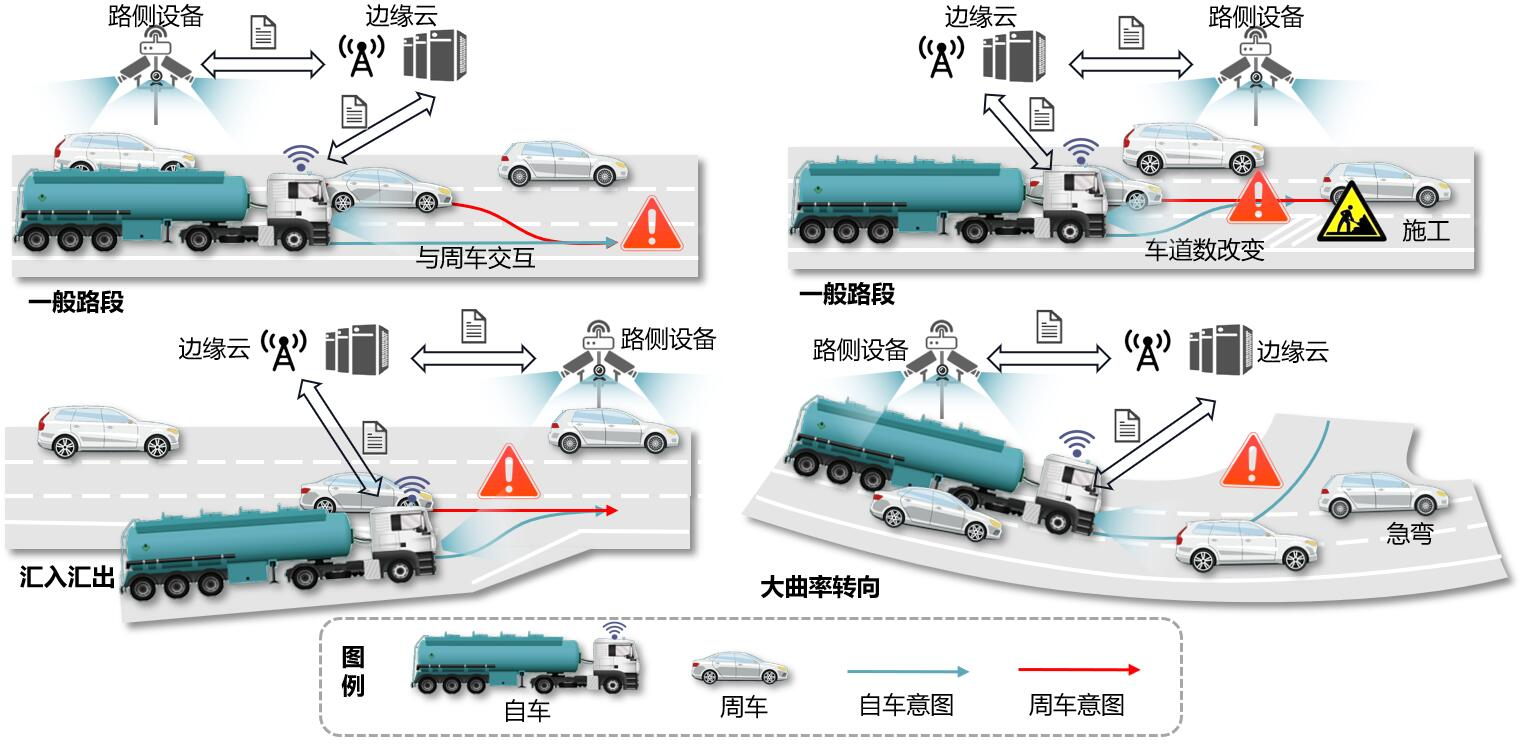
\includegraphics[width=0.9\linewidth]{fig/chap1/use_case.jpg}
      \caption{研究对象示意图}
      \label{fig:use_case}
    \end{figure}

    研究场景面向高等级公路典型运行环境，重点考虑液罐车侧翻风险较高的高速公路全路段及部分路口/匝道场景，包括一般路段、上/下匝道、大曲率弯道、施工区域、车道数变化等典型工况，并考虑目标液罐车与周车之间的动态交互。

    本文聚焦自动驾驶半挂式液罐车，是因为半挂式液罐车在危化品运输中占比高、载重大、质心高、操纵与稳定控制更为复杂，具有更突出的防侧翻研究意义。本文假设目标车辆具备基本的环境感知、决策规划与闭环控制能力。

    本文的研究目标是充分发挥云控系统广域感知与并行计算优势，将云端预测性风险规避与车端实时安全保障相结合，在兼顾通行效率与运行经济性的前提下，提高液罐车行驶过程中的侧翻稳定性并降低进入危险状态的概率。




\subsection{总体研究方案}

  针对上述问题，本文围绕“云端预测性规避风险、车端实时性保障安全”的总体思路，构建车云协同液罐车防侧翻行驶规划与控制总体方案。整体上，本文按照“体系架构设计—云端预测性决策规划—车端防侧翻控制—验证评估”的主线展开研究，目标是在发挥云端全局感知与计算优势的同时，保留车端快速闭环与安全兜底能力，形成“云端风险前移—车端局部执行—控制层极限兜底”的分层防控机制。

  \begin{figure}
    \centering
    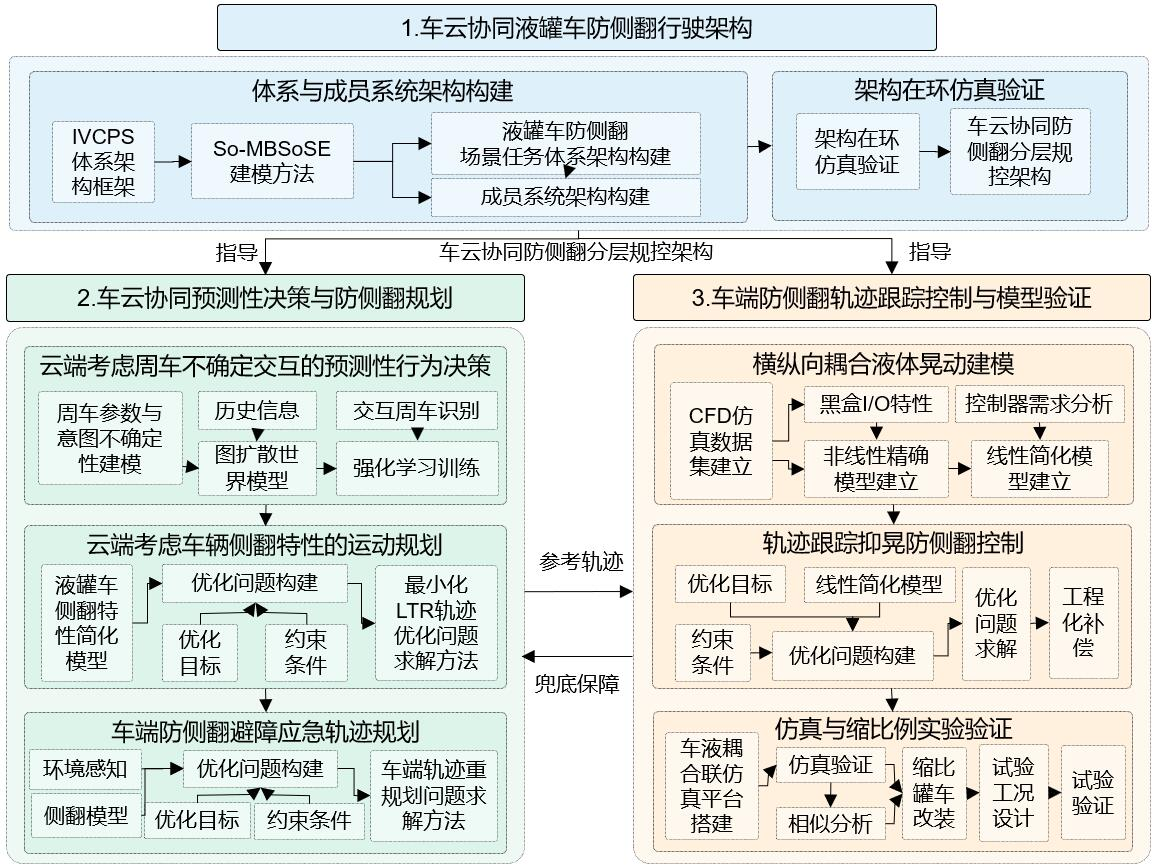
\includegraphics[width=1.0\linewidth]{fig/chap1/architecture.jpg}
    \caption{本文研究框架}
    \label{fig:thesis_archi}
  \end{figure}


  首先，从体系架构层面明确车端、云端与通信链路在防侧翻任务中的功能边界、协同关系并建立运行安全保障机制，形成面向液罐车防侧翻的车云协同总体架构。

  其次，从云端决策规划层面，利用广域感知与并行计算优势开展长时域风险预判与预测性规避，为车辆提供面向防侧翻任务的先验决策引导与参考轨迹支持。

  再次，从车端执行层面，面向局部实时约束与临险工况，构建具有防侧翻能力的规划控制方法，使车辆在跟踪上层参考的同时保持侧倾稳定性，并在云端建议失效或场景突变时提供安全兜底。

  最后，从验证评估层面，面向防侧翻任务进行车液耦合仿真与模型车实验验证评估，对所提出的方法进行评估，形成从理论设计到验证闭环的完整支撑。




